\section{Proof the Theorem}
$(\Rightarrow)$  Nếu đồ thị $G$ chứa đồ thị con là subdivision của $K_5$ hoặc $K_{3,3}$ thì $G$ không phẳng. \\

\begin{proof}
    Ta có:
    \begin{itemize}
        \item Subdivision của đồ thị không phẳng thì không phẳng

        \item Nếu một đồ thị con không phẳng thì đồ thị không phẳng

        \item Nếu một đồ thị con của đồ thị $G$ là subdivision của đồ thị không phẳng thì $G$ không phẳng
    \end{itemize}
    \begin{lemma}
        $K_{3,3}$ is không phẳng
    \end{lemma}

    \begin{proof}
        Chúng ta sẽ chứng minh bằng phản chứng.

        Giả sử tồn tại một biểu diễn phẳng của $K_{3,3}$. Trong đồ thị phân đôi đơn, chiều dài nhỏ nhất của chu trình là 4, nghĩa là với mọi $f \in F(K_{3,3})$
        $$deg(f) \geq 4$$
        Lại có $$\sum_{f \in F(K_{3,3})}deg(f) = 2\epsilon$$
        \begin{figure}[H]
            \begin{minipage}{0.3\textwidth}
                $$V-E+F=2$$
                $$6-E+F=2$$
                $$6-9+F=2$$
                $$F=5$$
            \end{minipage}
            \hfill
            \begin{minipage}{0.35\textwidth}
                \centering
                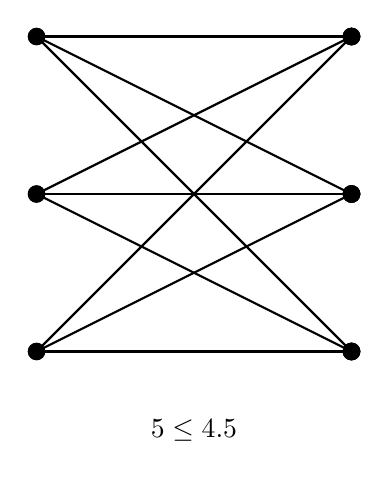
\begin{tikzpicture}
                    \foreach \x/\y in {0/1, 0/3, 0/5} {
                            \filldraw[black] (\x,\y) circle (3pt);
                            \foreach \z/\t in {4/1, 4/3, 4/5} {
                                    \filldraw[black] (\z,\t) circle (3pt);
                                    \draw[black, thick] (\x,\y) -- (\z,\t);
                                }
                        }
                    \node at (2,0,0) {$5 \leq 4.5$};
                \end{tikzpicture}
            \end{minipage}
            \hfill
            \begin{minipage}{0.3\textwidth}
                \centering
                % No 3 edge faces
                $$4F \leq 2E$$
                $$4F \leq 2 \times 9$$
                $$ F \leq 4.5$$
            \end{minipage}
        \end{figure}
    \end{proof}

    \begin{lemma}
        $K_5$ is không phẳng
    \end{lemma}
    \begin{proof}
        Giả sử tồn tại một biểu diễn phẳng của $K_{3,3}$. Trong đồ thị phân đôi đơn, chiều dài nhỏ nhất của chu trình là 4, nghĩa là với mọi $f \in F(K_{3,3})$
        $$deg(f) \geq 3$$
        Lại có $$\sum_{f \in F(K_{3,3})}deg(f) = 2\epsilon$$
        \begin{figure}[H]
            \begin{minipage}{0.3\textwidth}
                $$V-E+F=2$$
                $$5-E+F=2$$
                $$5-10+F=2$$
                $$F=7$$
            \end{minipage}
            \hfill
            \begin{minipage}{0.35\textwidth}
                \centering
                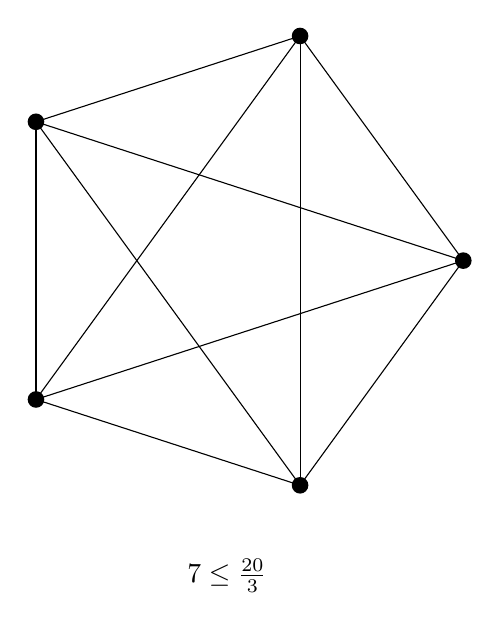
\begin{tikzpicture}
                    \foreach \i in {1, 2, 3, 4, 5}
                    \fill[black] (\i*360/5:3) coordinate (5\i) circle(3 pt)
                    \ifnum \i>1 foreach \j in {\i,...,1}{(5\i) edge (5\j)} \fi;

                    \node at (0,-4,0) {$7 \leq \frac{20}{3}$};
                \end{tikzpicture}
            \end{minipage}
            \hfill
            \begin{minipage}{0.3\textwidth}
                \centering
                $$3F \leq 2E$$
                $$3F \leq 2 \times 10$$
                $$F \leq \frac{20}{3}$$
            \end{minipage}
        \end{figure}
    \end{proof}
    \begin{recap}
    \end{recap}
    $K_5$ và $K_{3,3}$ là không phẳng

    $\Rightarrow$ Tất cả subdivisions của chúng đều không phẳng

    $\Rightarrow$ Nếu đồ thị $G$ chứa đồ thị con là subdivision của $K_5$ hoặc $K_{3,3}$ thì G không phẳng \\

\end{proof}
$(\Leftarrow)$ Nếu đồ thị $G$ không phẳng thì $G$ chứa subdivision của $K_5$ hoặc $K_{3,3}$
\begin{proof}
    Giả sử tồn tại đồ thị không phẳng mà không chứa đồ thị con là subdivisions của $K_5$ hoặc $K_{3,3}$.

    Cho $G$ là đồ thị không phẳng \textit{cực tiểu}. Khi loại bỏ một cạnh bất kì của $G$ thì ta được đồ thị \textit{phẳng}.

    \begin{enumerate}
        \item $G$ là 2-connected
              \begin{proof}
                  \begin{center}
                      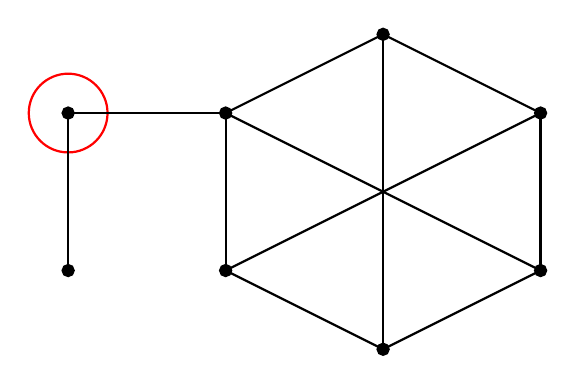
\begin{tikzpicture}
                          \draw[red, thick] (-2,3) circle (0.5);
                          \foreach \x/\y in {0/1, 2/0, 4/1, 0/3, 4/3, 2/4} {
                                  \filldraw[black, thick] (\x,\y) circle (2pt);
                                  \draw[black, thick] (2,2) -- (\x,\y);
                              }
                          \filldraw[black, thick] (-2,3) circle (2pt);
                          \filldraw[black, thick] (-2,1) circle (2pt);

                          \draw[black, thick] (0,1) -- (2,0);
                          \draw[black, thick] (2,0) -- (4,1);
                          \draw[black, thick] (4,1) -- (4,3);
                          \draw[black, thick] (0,3) -- (0,1);
                          \draw[black, thick] (4,3) -- (2,4);
                          \draw[black, thick] (2,4) -- (0,3);

                          \draw[black, thick] (-2,1) -- (-2,3);
                          \draw[black, thick] (-2,3) -- (0,3);

                      \end{tikzpicture}
                  \end{center}
                  Đầu tiên, ta chỉ ra $G$ 1-connected (liên thông). Giả sử $G$ không liên thông, và không phẳng.
                  Vì $G$ là đồ thị không phẳng cực tiểu nên các thành phần của nó là phẳng. Không mất tính tổng quát, giả sử G có 2 thành phần liên thông là $G_1$ và $G_2$.
                  Bởi vì $G_1$ và $G_2$ cùng phẳng, ta có thể thêm biểu diễn phẳng của $G_1$ vào một trong các diện biểu diễn phẳng của $G_2$ (ví dụ diện vô hạn), cho ta biểu diễn phẳng của $G$. Vô lý.

                  Vì $G$ liên thông nên $\kappa(G) \geq 1$. Giả sử $\kappa(G) = 1$, theo định nghĩa, tồn tại đỉnh $v$ sao cho $G -v$ không liên thông.
                  Không mất tính tổng quát, giả sử $G-v$ có 2 thành phần liên thông $H_1$ và $H_2$.
                  Ta có $H_1 \cup v$ và $H_2 \cup v$ đều phẳng vì tính cực tiểu của $G$.
                  Trong biểu diễn phẳng của chúng, ta có thể tìm một diện $f$ mà biên chứa đỉnh $v$.
                  Với phép chiếu lập thể, ta có thể thu được biểu diễn phẳng của $H_1 \cup v$ và $H_2 \cup v$ mà $v$ nằm trên đường biên của diện không bị chặn.
                  Bằng cách đặt điểm ở vô cùng.
                  Sau đó, ta gộp $H_1 \cup v$ và $H_2 \cup v$ bằng cách hợp nhất $v$ và thu được một biểu diễn phẳng của G. Vô lý.

                  Vậy, nếu $G$ là đồ thị không phẳng cực tiểu thì $G$ 2-connected.

              \end{proof}
        \item $deg(v) \geq 3$ for all vertex $v$ in $G$

              Chứng minh phản chứng: assume some vertex $v \in G$ has $deg(v) \leq 2$

        \item Nếu $G$ là đồ thị không phẳng \textit{cực tiểu} thì tồn tại $uv$ để $G-uv$ 2-connected
              \begin{proof}
                  Vì $G$ 2-connected nên $\kappa(G) \geq 2$. Giả sử $\kappa(G) =2$ thì tồn tại 2 đỉnh $u,v$ sao cho $G-\{u,v\}$ không liên thông.
                  Gọi các thành phần liên thông của $G-\{u,v\}$ là $H_1, H_2, \ldots,H_k$. Xây dựng tập $M_1,M_2,\ldots,M_k$ trọng đó $M_i=H_i \cup \{u,v\} +uv$.
                  Ta sẽ chỉ ra tồn tại $M_i (1 \geq i \geq k)$ không phẳng.

                  Giả sử tất cả $M_i (1 \geq i \geq k)$ đều phẳng, do đó tồn tại biểu diễn phẳng của mỗi chúng.
                  Vì $\{u,v\}$ và $uv$ là phân chung duy nhất của các $M_i$, do đó, ta có thể hợp nhất biểu diễn phẳng của chúng, thu được biểu diễn phẳng của $G+uv$
                  Nghĩa là $G+uv$ phẳng, nên $G$ cũng phẳng. Vô lý, do đó tồn tại $M_j (1 \geq j \geq k)$ không phẳng.

                  Dễ thầy $\epsilon(M_j) < \epsilon(G)$. Vì $G$ là đồ thị cực tiểu không chứa subdivision $K_5$ và $K_{3,3}$

              \end{proof}
              \begin{tikzpicture}

              \end{tikzpicture}
    \end{enumerate}

\end{proof}

Take the egde $uv$ from the previous statement, and consider the đồ thị $G-uv$ obtained by removing it

$G-uv$ is planar by minimality

$G-uv$ is 2-connected, so there is a cycle contains $u,v$.

\begin{remark}
    Note that the edges we are drawing here are really paths in đồ thị
\end{remark}

\begin{figure}[H]
    \begin{minipage}{0.4\textwidth}
        \begin{tikzpicture}
            \draw[black, thick] (0,0) circle (3);
            \filldraw[black, thick] (-3,0) circle (2pt);
            \filldraw[black, thick] (3,0) circle (2pt);
            \node at (-3.5,0,0) {$u$};
            \node at (3.5,0,0) {$v$};
            \node at (0,2.5,0) {$C$};
        \end{tikzpicture}
    \end{minipage}
    \hfill
    \begin{minipage}{0.5\textwidth}
        Embeded maximal cycle $C$ containing $u,v$
    \end{minipage}

\end{figure}

\begin{figure}[H]
    \begin{minipage}{0.4\textwidth}
        \begin{tikzpicture}
            \draw[black, thick] (0,0) circle (3);
            \filldraw[black, thick] (-3,0) circle (2pt);
            \filldraw[black, thick] (3,0) circle (2pt);
            \node at (-3.5,0,0) {$u$};
            \node at (3.5,0,0) {$v$};
            \node at (0,2.5,0) {$C$};
        \end{tikzpicture}
    \end{minipage}
    \hfill
    \begin{minipage}{0.5\textwidth}
        We embeded $G -uv$ so that $C$ enclose more regions of the đồ thị than any other cycle containing $u$ and $v$ could
    \end{minipage}

\end{figure}

\begin{figure}[H]
    \begin{minipage}{0.4\textwidth}
        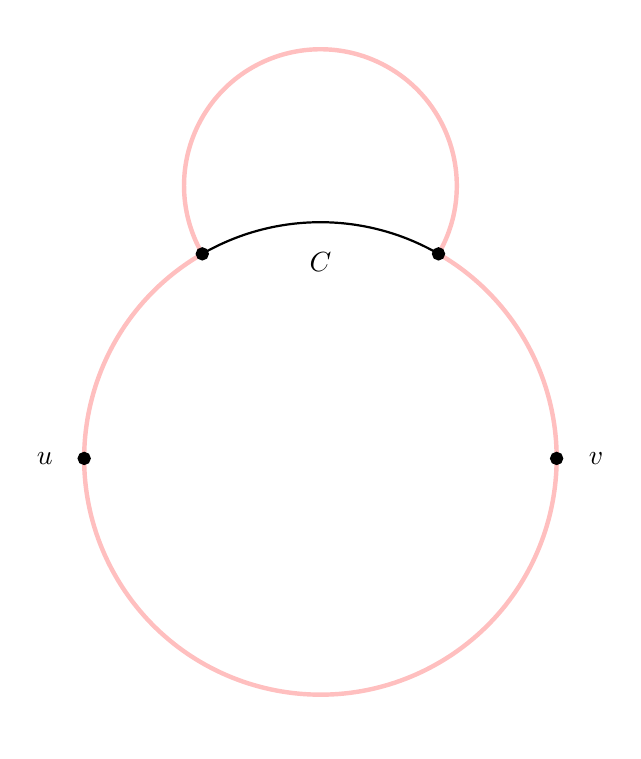
\begin{tikzpicture}
            \draw[pink, ultra thick] (1.5,{sqrt(27/4)}) arc (-30:210:{sqrt(3)});
            \draw[black, thick] (1.5,{sqrt(27/4)}) arc (60:120:3);
            \draw[pink, ultra thick] (-1.5,{sqrt(27/4)}) arc (120:420:3);
            \filldraw[black, thick] (1.5,{sqrt(27/4)}) circle (2pt);
            \filldraw[black, thick] (-1.5,{sqrt(27/4)}) circle (2pt);
            \filldraw[black, thick] (-3,0) circle (2pt);
            \filldraw[black, thick] (3,0) circle (2pt);

            \node at (-3.5,0,0) {$u$};
            \node at (3.5,0,0) {$v$};
            \node at (0,2.5,0) {$C$};
        \end{tikzpicture}
    \end{minipage}
    \hfill
    \begin{minipage}{0.4\textwidth}
        Loop along upper or lower part of $C$?

        We can't have any extra paths on the upper or lower part of $C$ since then there would be a cycle which contains more regions

        Larger cycle $\Rightarrow$ Contradiction
    \end{minipage}

\end{figure}


\begin{figure}[H]
    \begin{minipage}{0.4\textwidth}
        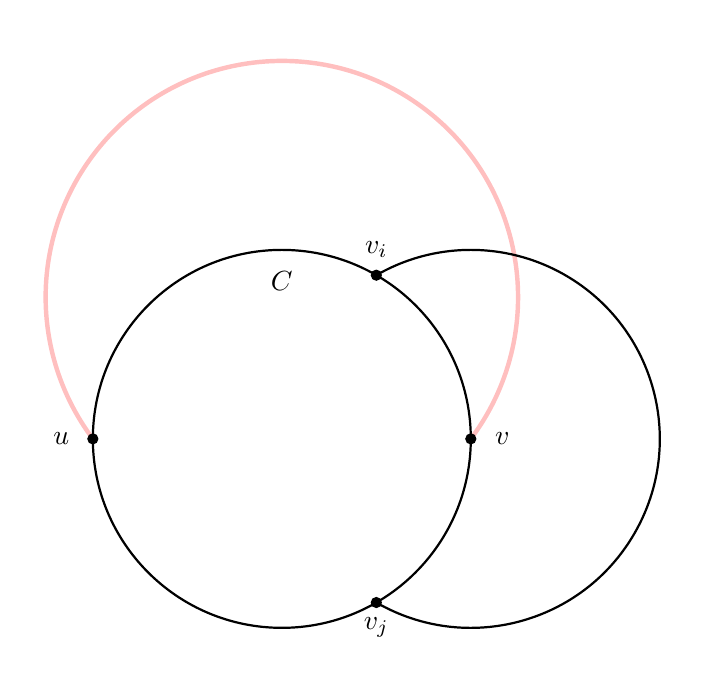
\begin{tikzpicture}[scale = 0.8]
            \draw[black, thick] (0,0) circle (3);
            \draw[pink, ultra thick] (3,0) arc (-acos(3/3.75):180+acos(3/3.75):3.75);
            \draw[black, thick] (1.5,-{sqrt(27/4)}) arc (-120:120:3);

            \filldraw[black, thick] (-3,0) circle (2pt);
            \filldraw[black, thick] (3,0) circle (2pt);
            \filldraw[black, thick] (1.5,{sqrt(27/4)}) circle (2pt);
            \filldraw[black, thick] (1.5,-{sqrt(27/4)}) circle (2pt);
            \node at (1.5,3,0) {$v_i$};
            \node at (1.5,-3,0) {$v_j$};
            \node at (-3.5,0,0) {$u$};
            \node at (3.5,0,0) {$v$};
            \node at (0,2.5,0) {$C$};
        \end{tikzpicture}
    \end{minipage}
    \hfill
    \begin{minipage}{0.4\textwidth}
        $G$ is không phẳng, so we need an osbtruction to $uv$ on the outside of $C$. There must exist a path $v_iv_j$ that blocks $uv$
    \end{minipage}
\end{figure}

The inside of $C$ must contain an obstruction. This obstruction also has to block $v_iv_j$ from being draw inside of $C$ since otherwise we could just draw it inside and draw $uv$ on the outside.

Up to equivalence there are only four types of obstructions we could draw here. \\

\begin{figure}[H]
    \begin{minipage}{0.4\textwidth}
        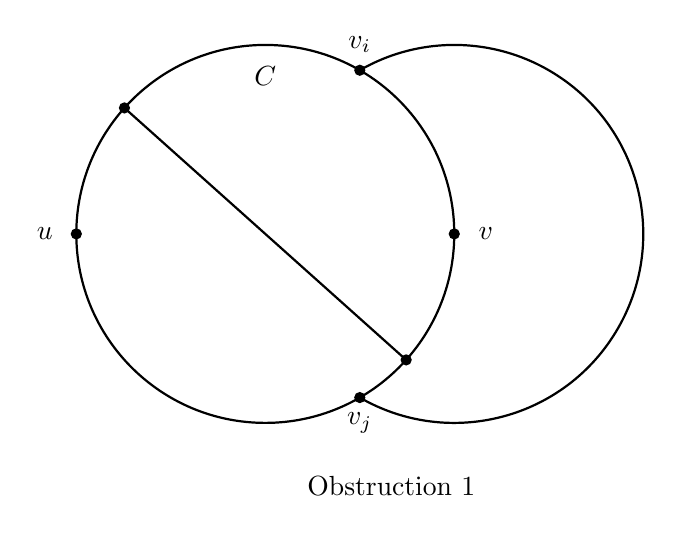
\begin{tikzpicture}[scale = 0.8]
            \draw[black, thick] (0,0) circle (3);
            \draw[black, thick] (1.5,-{sqrt(27/4)}) arc (-120:120:3);
            \draw[black, thick] ({-sqrt(5)},2) -- ({sqrt(5)},-2);
            \filldraw[black, thick] (-3,0) circle (2pt);
            \filldraw[black, thick] (3,0) circle (2pt);
            \filldraw[black, thick] ({-sqrt(5)},2) circle (2pt);
            \filldraw[black, thick] ({sqrt(5)},-2) circle (2pt);
            \filldraw[black, thick] (1.5,{sqrt(27/4)}) circle (2pt);
            \filldraw[black, thick] (1.5,-{sqrt(27/4)}) circle (2pt);
            \node at (1.5,3,0) {$v_i$};
            \node at (1.5,-3,0) {$v_j$};
            \node at (-3.5,0,0) {$u$};
            \node at (3.5,0,0) {$v$};
            \node at (0,2.5,0) {$C$};

            \node at (2,-4,0) {Obstruction 1};
        \end{tikzpicture}
    \end{minipage}
    \hfill
    \begin{minipage}{0.4\textwidth}
        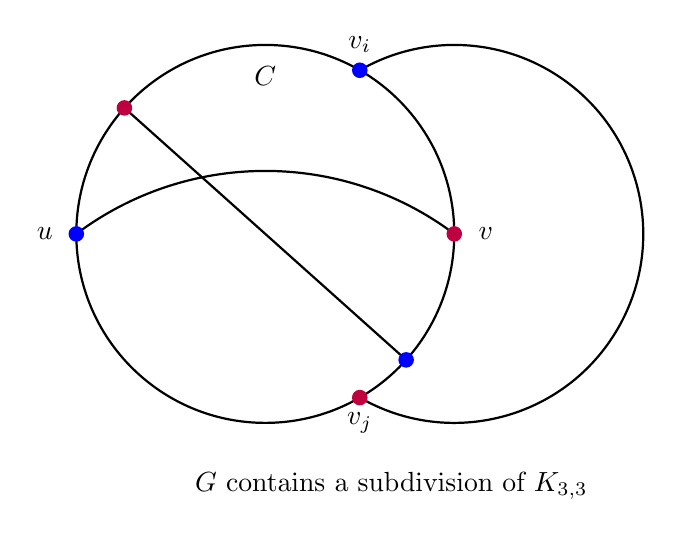
\begin{tikzpicture}[scale = 0.8]
            \draw[black, thick] (0,0) circle (3);
            \draw[black, thick] (1.5,-{sqrt(27/4)}) arc (-120:120:3);
            \draw[black, thick] (3,0) arc (acos(0.6):180-acos(0.6):5);
            \draw[black, thick] ({sqrt(5)},-2) -- (-{sqrt(5)},2);
            \filldraw[blue, thick] (-3,0) circle (3pt);
            \filldraw[purple, thick] (3,0) circle (3pt);
            \filldraw[purple, thick] ({-sqrt(5)},2) circle (3pt);
            \filldraw[blue, thick] ({sqrt(5)},-2) circle (3pt);
            \filldraw[blue, thick] (1.5,{sqrt(27/4)}) circle (3pt);
            \filldraw[purple, thick] (1.5,-{sqrt(27/4)}) circle (3pt);
            \node at (1.5,3,0) {$v_i$};
            \node at (1.5,-3,0) {$v_j$};
            \node at (-3.5,0,0) {$u$};
            \node at (3.5,0,0) {$v$};
            \node at (0,2.5,0) {$C$};
            \node at (2,-4,0) {$G$ contains a subdivision of $K_{3,3}$};

        \end{tikzpicture}
    \end{minipage}
\end{figure}

\begin{figure}[H]
    \begin{minipage}{0.4\textwidth}
        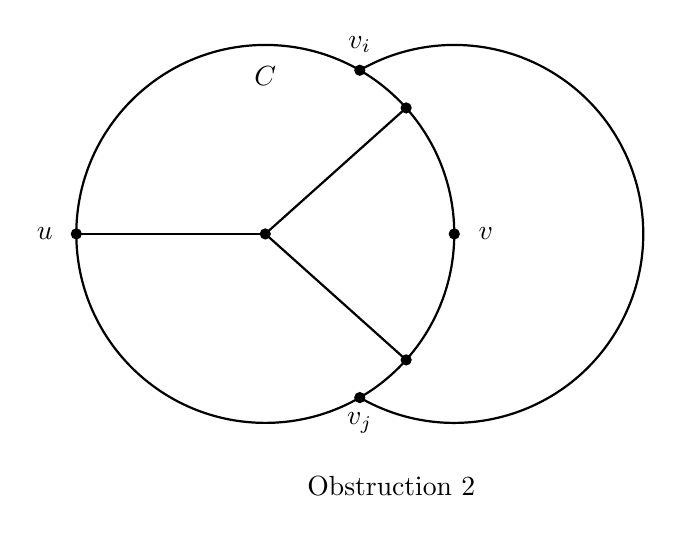
\begin{tikzpicture}[scale = 0.8]
            \draw[black, thick] (0,0) circle (3);
            \draw[black, thick] (1.5,-{sqrt(27/4)}) arc (-120:120:3);
            \draw[black, thick] (0,0) -- ({sqrt(5)},-2);
            \draw[black, thick] (0,0) -- ({sqrt(5)},2);
            \draw[black, thick] (0,0) -- (-3,0);
            \filldraw[black, thick] (-3,0) circle (2pt);
            \filldraw[black, thick] (3,0) circle (2pt);
            \filldraw[black, thick] (0,0) circle (2pt);
            \filldraw[black, thick] ({sqrt(5)},2) circle (2pt);
            \filldraw[black, thick] ({sqrt(5)},-2) circle (2pt);
            \filldraw[black, thick] (1.5,{sqrt(27/4)}) circle (2pt);
            \filldraw[black, thick] (1.5,-{sqrt(27/4)}) circle (2pt);
            \node at (1.5,3,0) {$v_i$};
            \node at (1.5,-3,0) {$v_j$};
            \node at (-3.5,0,0) {$u$};
            \node at (3.5,0,0) {$v$};
            \node at (0,2.5,0) {$C$};

            \node at (2,-4,0) {Obstruction 2};
        \end{tikzpicture}
    \end{minipage}
    \hfill
    \begin{minipage}{0.4\textwidth}
        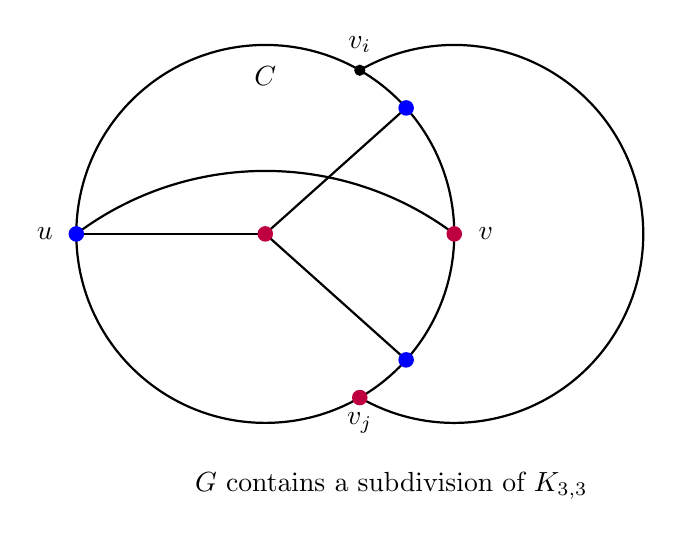
\begin{tikzpicture}[scale = 0.8]
            \draw[black, thick] (0,0) circle (3);
            \draw[black, thick] (1.5,-{sqrt(27/4)}) arc (-120:120:3);
            \draw[black, thick] (3,0) arc (acos(0.6):180-acos(0.6):5);
            \draw[black, thick] (0,0) -- ({sqrt(5)},-2);
            \draw[black, thick] (0,0) -- ({sqrt(5)},2);
            \draw[black, thick] (0,0) -- (-3,0);
            \filldraw[blue, thick] (-3,0) circle (3pt);
            \filldraw[purple, thick] (3,0) circle (3pt);
            \filldraw[purple, thick] (0,0) circle (3pt);
            \filldraw[blue, thick] ({sqrt(5)},2) circle (3pt);
            \filldraw[blue, thick] ({sqrt(5)},-2) circle (3pt);
            \filldraw[black, thick] (1.5,{sqrt(27/4)}) circle (2pt);
            \filldraw[purple, thick] (1.5,-{sqrt(27/4)}) circle (3pt);
            \node at (1.5,3,0) {$v_i$};
            \node at (1.5,-3,0) {$v_j$};
            \node at (-3.5,0,0) {$u$};
            \node at (3.5,0,0) {$v$};
            \node at (0,2.5,0) {$C$};
            \node at (2,-4,0) {$G$ contains a subdivision of $K_{3,3}$};

        \end{tikzpicture}
    \end{minipage}
\end{figure}

\begin{figure}[H]
    \begin{minipage}{0.4\textwidth}
        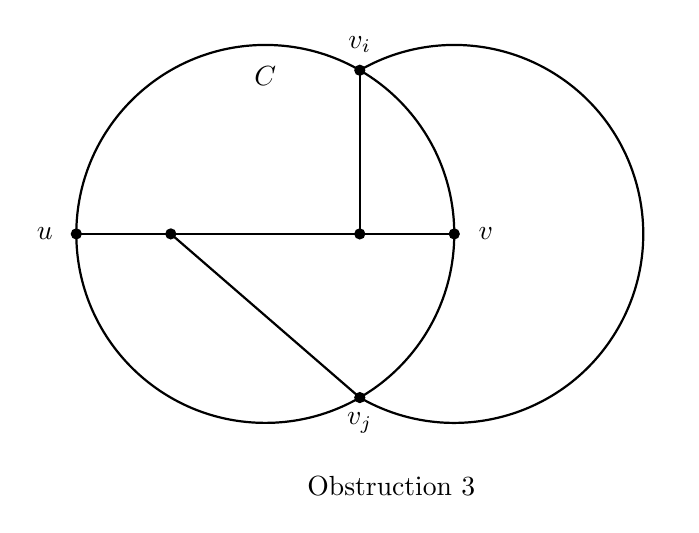
\begin{tikzpicture}[scale = 0.8]
            \draw[black, thick] (0,0) circle (3);
            \draw[black, thick] (1.5,-{sqrt(27/4)}) arc (-120:120:3);
            \draw[black, thick] (3,0) -- (-3,0);
            \draw[black, thick] (1.5,0) -- (1.5,{sqrt(27/4)});
            \draw[black, thick] (-1.5,0) -- (1.5,-{sqrt(27/4)});
            \filldraw[black, thick] (-3,0) circle (2pt);
            \filldraw[black, thick] (3,0) circle (2pt);
            \filldraw[black, thick] (1.5,{sqrt(27/4)}) circle (2pt);
            \filldraw[black, thick] (1.5,-{sqrt(27/4)}) circle (2pt);
            \filldraw[black, thick] (1.5,0) circle (2pt);
            \filldraw[black, thick] (-1.5,0) circle (2pt);
            \node at (1.5,3,0) {$v_i$};
            \node at (1.5,-3,0) {$v_j$};
            \node at (-3.5,0,0) {$u$};
            \node at (3.5,0,0) {$v$};
            \node at (0,2.5,0) {$C$};

            \node at (2,-4,0) {Obstruction 3};
        \end{tikzpicture}
    \end{minipage}
    \hfill
    \begin{minipage}{0.4\textwidth}
        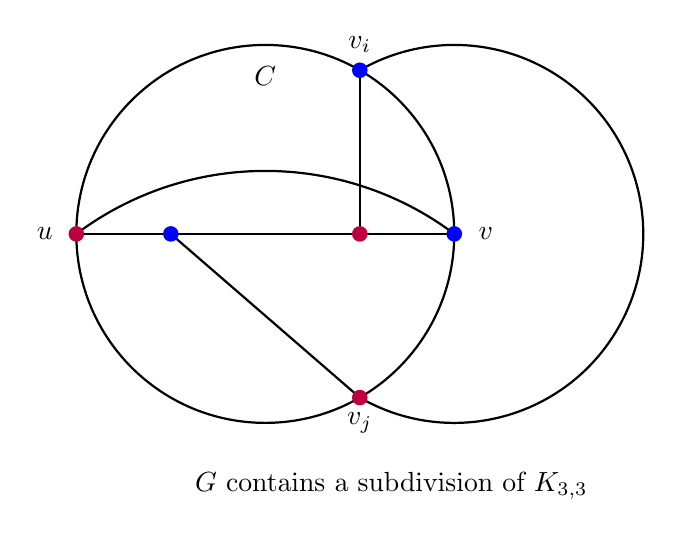
\begin{tikzpicture}[scale = 0.8]
            \draw[black, thick] (3,0) arc (acos(0.6):180-acos(0.6):5);
            \draw[black, thick] (0,0) circle (3);
            \draw[black, thick] (1.5,-{sqrt(27/4)}) arc (-120:120:3);
            \draw[black, thick] (3,0) -- (-3,0);
            \draw[black, thick] (1.5,0) -- (1.5,{sqrt(27/4)});
            \draw[black, thick] (-1.5,0) -- (1.5,-{sqrt(27/4)});
            \filldraw[purple, thick] (-3,0) circle (3pt);
            \filldraw[blue, thick] (3,0) circle (3pt);
            \filldraw[blue, thick] (1.5,{sqrt(27/4)}) circle (3pt);
            \filldraw[purple, thick] (1.5,-{sqrt(27/4)}) circle (3pt);
            \filldraw[purple, thick] (1.5,0) circle (3pt);
            \filldraw[blue, thick] (-1.5,0) circle (3pt);
            \node at (1.5,3,0) {$v_i$};
            \node at (1.5,-3,0) {$v_j$};
            \node at (-3.5,0,0) {$u$};
            \node at (3.5,0,0) {$v$};
            \node at (0,2.5,0) {$C$};
            \node at (2,-4,0) {$G$ contains a subdivision of $K_{3,3}$};

        \end{tikzpicture}
    \end{minipage}
\end{figure}


\begin{figure}[H]
    \begin{minipage}{0.4\textwidth}
        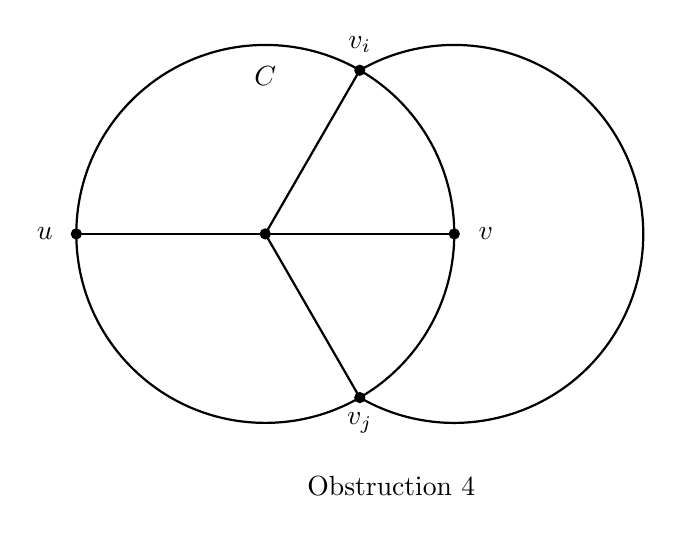
\begin{tikzpicture}[scale = 0.8]
            \draw[black, thick] (0,0) circle (3);
            \draw[black, thick] (1.5,-{sqrt(27/4)}) arc (-120:120:3);
            \draw[black, thick] (3,0) -- (-3,0);
            \draw[black, thick] (0,0) -- (1.5,{sqrt(27/4)});
            \draw[black, thick] (0,0) -- (1.5,-{sqrt(27/4)});
            \filldraw[black, thick] (-3,0) circle (2pt);
            \filldraw[black, thick] (3,0) circle (2pt);
            \filldraw[black, thick] (1.5,{sqrt(27/4)}) circle (2pt);
            \filldraw[black, thick] (1.5,-{sqrt(27/4)}) circle (2pt);
            \filldraw[black, thick] (0,0) circle (2pt);
            \node at (1.5,3,0) {$v_i$};
            \node at (1.5,-3,0) {$v_j$};
            \node at (-3.5,0,0) {$u$};
            \node at (3.5,0,0) {$v$};
            \node at (0,2.5,0) {$C$};

            \node at (2,-4,0) {Obstruction 4};
        \end{tikzpicture}
    \end{minipage}
    \hfill
    \begin{minipage}{0.4\textwidth}
        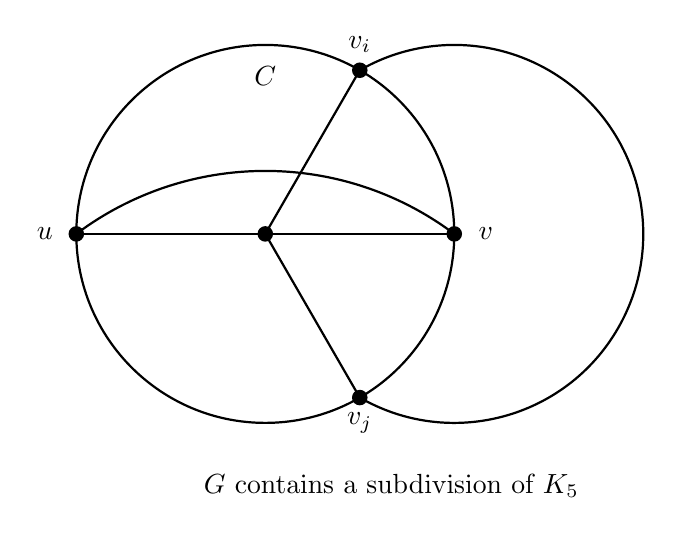
\begin{tikzpicture}[scale = 0.8]
            \draw[black, thick] (3,0) arc (acos(0.6):180-acos(0.6):5);
            \draw[black, thick] (0,0) circle (3);
            \draw[black, thick] (1.5,-{sqrt(27/4)}) arc (-120:120:3);
            \draw[black, thick] (3,0) -- (-3,0);
            \draw[black, thick] (0,0) -- (1.5,{sqrt(27/4)});
            \draw[black, thick] (0,0) -- (1.5,-{sqrt(27/4)});
            \filldraw[black, thick] (-3,0) circle (3pt);
            \filldraw[black, thick] (3,0) circle (3pt);
            \filldraw[black, thick] (1.5,{sqrt(27/4)}) circle (3pt);
            \filldraw[black, thick] (1.5,-{sqrt(27/4)}) circle (3pt);
            \filldraw[black, thick] (0,0) circle (3pt);
            \node at (1.5,3,0) {$v_i$};
            \node at (1.5,-3,0) {$v_j$};
            \node at (-3.5,0,0) {$u$};
            \node at (3.5,0,0) {$v$};
            \node at (0,2.5,0) {$C$};
            \node at (2,-4,0) {$G$ contains a subdivision of $K_5$};

        \end{tikzpicture}
    \end{minipage}
\end{figure}
\begin{remark}
    $G$ always contains a subđồ thị which is subdivisionof $K_5$ or $K_{3,3}$
\end{remark}
In all of the four cases the result is a 4 cases, the result is a contradiction. We assume that $G$ contained at neither of the two đồ thịs. With this, we are left to conclude that there are no không phẳng đồ thịs like $G$. This proves the theorem.
